\documentclass{article}
\usepackage[margin=1in]{geometry}
\usepackage{amsmath,amsthm,amssymb}
\usepackage{bbm,enumerate,mathtools}
\usepackage{tikz,pgfplots}
\usepackage{chessboard}
\usepackage[hidelinks]{hyperref}
\usepackage{multicol} % Problem 35
\usepackage{xstring} % Difficulty command
\usetikzlibrary{shapes.geometric}

\newenvironment{question}{\begin{trivlist}\item[\textbf{Question.}]}{\end{trivlist}}
\newenvironment{note}{\begin{trivlist}\item[\textbf{Note.}]}{\end{trivlist}}
\newenvironment{references}{\begin{trivlist}\item[\textbf{References.}]}{\end{trivlist}}
\newenvironment{related}{\begin{trivlist}\item[\textbf{Related.}]\end{trivlist}\begin{enumerate}}{\end{enumerate}}

\newcommand\score[1]{
\pgfmathsetmacro\pgfxa{#1+1}
\tikzstyle{scorestars}=[
  star,
  star points=5,
  star point ratio=2.25,
  draw,
  inner sep=3pt,
  anchor=outer point 5
]
  \begin{tikzpicture}[baseline]
    \draw[opacity=0] (0,-0.5) rectangle (0,0.2); % Workaround for whitespace at the bottom.
    \foreach \i in {1,...,4} {
      \pgfmathparse{(\i<=#1?"yellow":"gray")}
      \edef\starcolor{\pgfmathresult}
      \draw (\i*4.5ex,0) node[name=star\i,scorestars,fill=\starcolor]  {};
    }
  \end{tikzpicture}
}

\newcommand{\difficulty}[1]{%
  \IfEqCase{#1}{%
      {1}{
        
\begin{tikzpicture}[scale=0.7, baseline=0.9mm]%
          \definecolor{slopegreen}{rgb}{0.0, 0.5, 0.0}%
          \fill[slopegreen] (0.5,0.5) circle (0.5);%
        \end{tikzpicture}%
      }%
      {2}{
        
\begin{tikzpicture}[scale=0.7, baseline=0.9mm]%
          \definecolor{slopeblue}{rgb}{0.0, 0.44, 1.00}
          \fill[slopeblue] (0,0) rectangle (1,1);%
        \end{tikzpicture}%
      }%
      {3}{
\begin{tikzpicture}[scale=0.7, baseline=0.9mm]\fill (0,0.5)--(0.5, 0)--(1,0.5)--(0.5,1)--cycle; \end{tikzpicture}}%
      {4}{
\begin{tikzpicture}[scale=0.7, baseline=0.9mm]\fill (0.25,0)--(0,0.5)--(0.25,1)--(0.5,0.5)--cycle; \fill (0.75,0)--(0.5,0.5)--(0.75,1)--(1,0.5)--cycle;\end{tikzpicture}}%
      % you can add more cases here as desired
  }[\PackageError{difficulty}{Undefined difficulty level: #1}{}]%
}%
\newcommand{\rating}[2]{\difficulty{#1}\\\score{#2}\\}


\begin{document}
\rating{0}{1}
Consider labeled rooted trees where the sum of the labels of the branches
connected to a vertex is less than the parent label, and the ``top'' label is
$n$.
\begin{figure}[!h]
  \centering
  \begin{tikzpicture}
    \node {5}
      child { node {1} }
      child { node {1} }
      child { node {1} }
      child { node {1} };
  \end{tikzpicture}\hspace{0.5cm}
  \begin{tikzpicture}
    \node {5}
      child {
        node {2}
        child { node {1} }
      }
      child { node {1} }
      child { node {1} };
  \end{tikzpicture}\hspace{0.5cm}
  \begin{tikzpicture}
    \node {5}
      child {
        node {2}
        child { node {1} }
      }
      child {
        node {2}
        child { node {1} }
      };
  \end{tikzpicture}\hspace{0.5cm}
  \begin{tikzpicture}
    \node {5}
      child {
        node {3}
        child { node {1} }
        child { node {1} }
      }
      child { node {1} };
  \end{tikzpicture}\\~\\
  \begin{tikzpicture}
    \node {5}
      child {
        node {3}
        child {
          node {2}
          child { node {1} }
        }
      }
      child { node {1} };
  \end{tikzpicture}\hspace{0.5cm}
  \begin{tikzpicture}
    \node {5}
      child {
        node {4}
        child { node {1} }
        child { node {1} }
        child { node {1} }
      };
  \end{tikzpicture}\hspace{0.5cm}
  \begin{tikzpicture}
    \node {5}
      child {
        node {4}
        child {
          node {2}
          child { node {1} }
        }
        child { node {1} }
      };
  \end{tikzpicture}\hspace{0.5cm}
  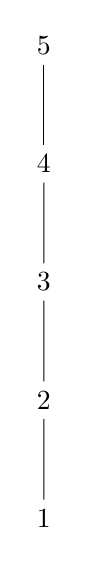
\begin{tikzpicture}
    \node {5}
      child {
        node {4}
        child {
          node {3}
          child {
            node {2}
            child { node {1} }
          }
        }
      };
  \end{tikzpicture}
  \caption{
    Eight examples of trees with a greatest label of $5$:
    $a(5) = a(1)^4 + a(2)a(1)^2 + a(2)^2 + a(3)a(1) + a(4) = 8$
  }
\end{figure}
\begin{question}
  How many such labels exist?
\end{question}
\begin{related}
  \item What if the same label cannot appear multiple times in the same row?
  \item What if labels are strictly greater than $1$ and the \textit{product} of
    the branches is less than their parent?
\end{related}
\begin{references}
  \item \url{https://oeis.org/A196545}
\end{references}

\end{document}
